\begin{figure}[hbtp]
  \centering
  % \subfigure[Without using auxiliary information]{
  %   \label{fig:about-auxiliary--without}
  %   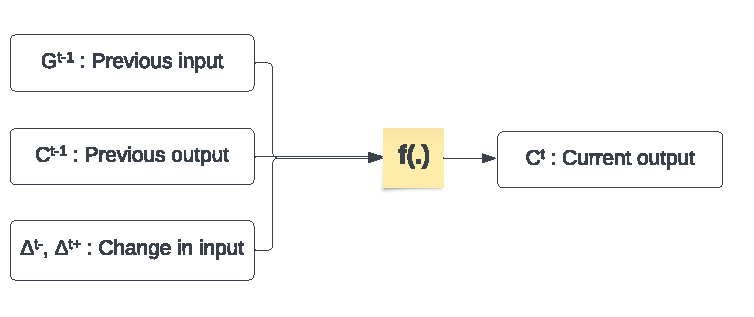
\includegraphics[width=0.48\linewidth]{out/about-auxiliary-without.pdf}
  % }
  \subfigure{
    \label{fig:about-auxiliary--with}
    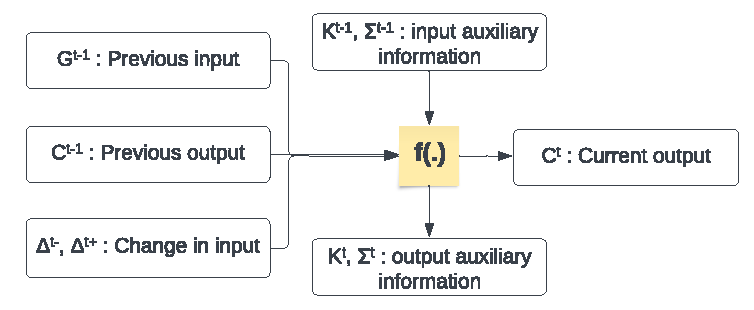
\includegraphics[width=0.98\linewidth]{out/about-auxiliary-with.pdf}
  } \\[-2ex]
  \caption{A dynamic community detection algorithm $f(.)$ accepts as input the previous graph $G^{t-1}$, community memberships $C^{t-1}$, and the batch update $\Delta^{t-}$, $\Delta^{t+}$, and returns the updated community memberships $C^t$. However\ignore{, as shown in (b)}, it may also accept weighted degree of vertices $K^{t-1}$ and total edge weights of communities $\Sigma^{t-1}$ as auxiliary information, and generate updated auxiliary information $K^t$, $\Sigma^t$.}
  \label{fig:about-auxiliary}
\end{figure}
